

\chapter[Socioeconomic and Health Consequences]{Socioeconomic and Health Consequences}
\label{cp:consequences}

\vspace{.935em}

The environmental collapse of the Aral Sea has had severe socioeconomic and health impacts on the surrounding communities, with lasting consequences for the people who depended on the lake for their livelihoods. 

\section{Loss of Jobs in the Fishing Industry}
One of the most immediate and dramatic impacts of the Aral Sea's depletion was the collapse of the local fishing industry. Prior to the crisis, the lake supported one of the largest fisheries in the Soviet Union, with more than 60,000 people employed in fishing and related industries \autocite{plotnikov_fauna}. \autoref{cp:aral-fishing}shows evidence of a successful fishing industry that once existed. However, as the water became increasingly saline and the fish population collapsed, these jobs were lost. Many families found themselves without work, leading to widespread poverty in the affected region \autocite{micklin1988desiccation}. 

\section{The Decline of Port Towns}
The environmental degradation of the Aral Sea has led to the near-total collapse of port towns that once played a crucial role in the region's economy. Moynaq, formerly a prominent fishing center in Uzbekistan, lay approximately 150 kilometers from the nearest body of water in 2023 \autocite{bardsley2023toxic}. The population of Moynaq (see \autoref{cp:moynaq}) has sharply decreased, with an estimated 100,000 residents migrating due to the environmental collapse, leaving behind roughly 18,000 people who face health challenges and extreme living conditions \autocite{mannaerts2022port}. The retreat of the sea has rendered the port obsolete, resulting in the abandonment of infrastructure and the loss of livelihoods. This trend is observed in other settlements along the former coastline, where the depletion of the Aral Sea has caused significant depopulation and the collapse of local economies. The Aral Ship Graveyard (\autoref{fig:aral-grave}), located near Moynaq, further illustrates the scale of environmental change, as abandoned ships now lie stranded in the desert, marking the extent of the region’s transformation.

\section{Toxic Dust Storms and Health Issues}
Perhaps the most insidious consequence of the Aral Sea's desiccation is the health impact of toxic dust storms referred to as \textit{`black blizzards'} \autocite{upperdarby2025geotext}. As the exposed lakebed dried, it became a source of hazardous dust and chemicals. Winds carried this dust across the surrounding regions, and it often contained toxic pesticides and heavy metals from the agricultural runoff. These dust storms have been linked to a sharp increase in respiratory diseases, including asthma, bronchitis, and other chronic illnesses. Additionally, the presence of pesticides and industrial pollutants has contributed to a rise in cancers and birth defects in the affected populations \autocite{whishwilson2002crisis}.

\begin{figure}
    \centering
    \fbox{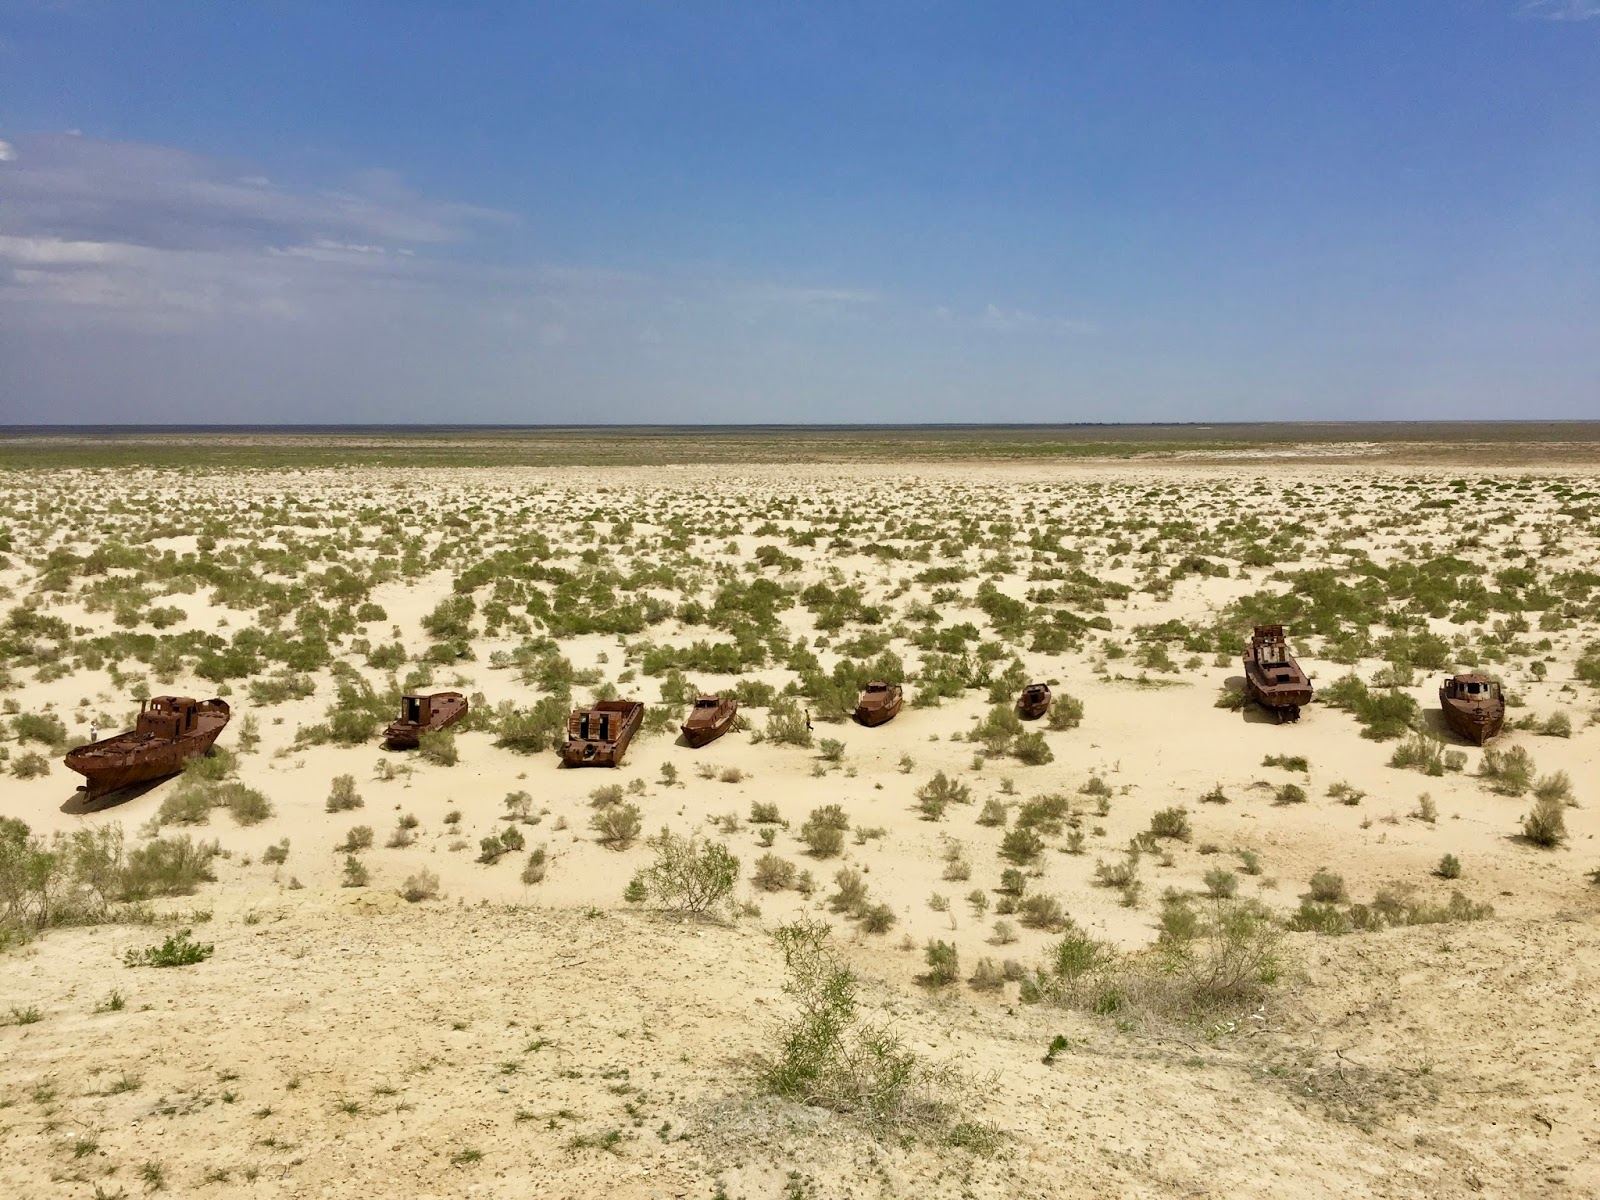
\includegraphics[width=0.8\linewidth]{Figures/Aral Ship Graveyard.png}}
    \caption{Aral Ship Graveyard}
    \label{fig:aral-grave}
\end{figure}

\section{Decline in Agricultural Productivity}
The degradation of the Aral Sea has also had a severe impact on local agriculture. As the lake receded, soil salinization increased, making it more difficult for farmers to grow crops. The irrigation systems that had been used to divert water from the rivers also led to a build-up of salts in the soil, further reducing its fertility. As a result, agricultural productivity in the surrounding areas plummeted, and many farmers have been forced to abandon their fields.
Between 1987 and 2019, approximately 3,129 $km^2$ of farmland in the Aral Sea region was abandoned due to salinization and desertification \autocite{shi2022farmland}. The scarcity of fresh water, combined with poor soil conditions, has further exacerbated the economic hardships faced by the region's agricultural workers \autocite{unesco2000vision}.

\section{Long-term Public Health Crisis}
The long-term health impacts of the Aral Sea crisis continue to affect the population today. The toxic environment, combined with the lack of economic opportunities, has created a public health crisis in the region. Diseases related to poor water quality, such as kidney and liver disease, have become increasingly common. Furthermore, the psychological toll of the
crisis, which has seen entire communities devastated, has led to increased mental health problems, including depression and anxiety \autocite{anchita2021health}.
